\section{Background and Key Contributions}

Fairness criteria quantify the relationship between the outcome metric across multiple subgroups or similar individuals in the population.
Formal definitions of fairness focus on observational criteria, i.e., those that can be written down as a probability statement involving the joint distribution of the features, sensitive attributes, decision-making function, and actual outcome.
Consider a decision-making function that claims to satisfy certain fairness guarantees.
In our setup, auditing a claim about a fairness guarantee would involve quantifying the probability of claim violations.
Given a particular failure probability $\Delta$ and a stream of data $\dots, (X_t, Y_t), \dots$ over time steps $t$ at run time, a fairness claim $\psi$ would be considered valid if $\Pr[\forall t \geq 1, \psi] \geq 1 - \Delta $.
Assuming that the data is sampled from a fixed, possibly unknown distribution $\pdata$, a common strategy to test the validity of a claim is to use hypothesis testing with a predetermined sample size $m$.
However, it is impossible to know a priori whether $m$ will be large enough to verify this hypothesis~\citep{waudby2021time}, and peeking at the data to determine the sample size would be considered `p-hacking.'
Collecting labeled data for fairness-related applications is expensive~\citep{ji2020can}; therefore, it is essential to ensure that a monitoring system used for auditing the fairness claim can \textit{adaptively and continuously update its estimates} of the probability of validity.
We consider a claim as invalid if $\Pr[\forall t \geq 1, \neg \psi] \geq 1 - \Delta$, where $\neg$ denotes negation.
Another desirable feature in the auditing system would be a \textit{finite-horizon stopping rule} that should be able to decide the validity/invalidity of a claim, given sufficient data.

We show that the framework of confidence sequences/sets~\cite{howard2021time} provides a mechanism for building confidence intervals for inference in sequential experiments with nonasymptotic (i.e., always valid for $t \geq 1$) intervals that approach zero width, ensuring that a stopping rule would have a finite termination.
We would also like to be able to \textit{localize and diagnose} terms within a fairness metric that leads to the inference of a negated claim.
For example, suppose $r \in \{ 0, 1\}$ denotes the return value of a binary decision function (say, job candidate selection), and $s$ is an indicator denoting whether a candidate belongs to a minority population.
The 80\%-rule for disparate impact~\citep{eeoc1979,feldman2015certifying} is a fairness criterion which states that
\begin{align*}
    \frac{\Pr[r=1| s]}{\Pr[r=1| \neg s]} \geq 0.8 
\end{align*}
Assuming that a confidence sequence approach leads to the inference of a negated claim (invalid) for disparate impact, a diagnosis would determine whether the numerator or denominator in the criterion lead to the invalidity.
\AVOIRmethodname{} uses an inference framework that builds upon distributional guarantees for each term within the criterion, which can help with such a diagnosis.
Further, overall uncertainty can be guaranteed across multiple groups by balancing it across subexpressions with differences in the number of observed samples.
For example, consider Bernoulli r.vs\footnote{random variables} $X_{1,2}$ for which we derive concentration guarantees $\Pr[|\E[X_i] - \BarE[X_i]| \geq \epsilon_{i}] \leq \delta_{i}$ after $t_{i}$ observations. 
Here, $\E[X]$ refers to the population mean, $\BarE[X]$ refers to an empirical mean based on observations of $X$, and $\epsilon, \delta > 0$ are the concentration level and failure probability, respectively.
From the Hoeffding inequality, $\delta = 2e^{-2t\epsilon^2}$.
We can claim tighter bounds for $X_2$ if $t_2 > t_1$ as the failure probability $\delta$ is lower at the same concentration $\epsilon$.
That is, $\eps_1 = \eps_2, t_2 > t_1 \Rightarrow \delta_1 > \delta_2$.
Varying $\epsilon$ across subexpressions to minimize the overall (union bounded) $\delta = \delta_1 + \delta_2$ allows an earlier stopping time for a valid/invalid claim, i.e., \textit{fewer iterations and fewer data samples}.
Adaptive versions of these inequalities also have similar patterns (see Figure~\ref{fig:n-comparison-hoeffding}).

\begin{figure}
    \centering
    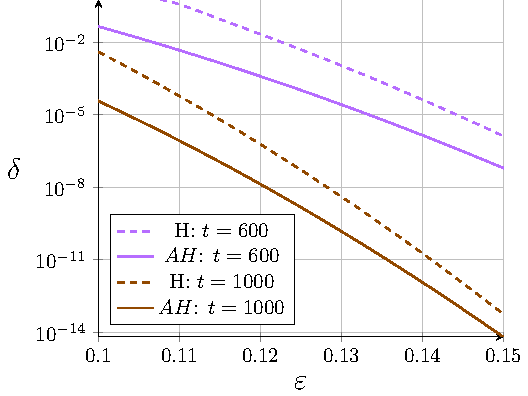
\includegraphics[width=0.75\linewidth]{avoir/images/bernoulli-n-comparison-pgf-tikz}
%    \resizebox{0.75\linewidth}{!}{
%        \newcommand*{\n}{}% Ensure it is not already defined
\newcommand*{\clr}{}% Ensure it is not already defined
\begin{tikzpicture}
                    \begin{axis}[
                            grid=both,
                            xlabel = {$\epsilon$},
                            x tick label style={/pgf/number format/fixed},
                            y tick label style={/pgf/number format/fixed},
                            ylabel = {$\delta$},
                            y label style={rotate=-90},
                            axis lines=left,
                            ymode=log,
                            xmin=0.1,
                            xmax=0.15,
                            legend style={at={(0.03,0.2)},anchor=west},
                            label style={font=\Large}
                    ]
                    \pgfplotsinvokeforeach{600/cb-lilac, 1000/cb-brown}
                    {       
                        \StrBefore{#1}{/}[\n]%
                        \StrBehind{#1}{/}[\clr]%
                        \edef\AddPlot{\noexpand\addplot[color=\clr,smooth,thick, dashed,-,domain=0:0.2] {min(2*\n*\n*exp(-2*\n*x*x), 1)};} %
                        \AddPlot
                        \addlegendentryexpanded{H: $t =\n$};
                        \edef\AddPlot{\noexpand\addplot[color=\clr,smooth,thick,-,domain=0:0.2] {min(24*(( (log10(\n)/log10(1.1)) + 1)^1.08)*(exp(-1.8*\n*x*x)), 1)};} %
                        \AddPlot
                        \addlegendentryexpanded{AH: $t =\n$};
                    }
                    \end{axis}
                    % https://tex.stackexchange.com/questions/325170/parameterizing-color-in-addplot
\end{tikzpicture}
%    }
    \caption{Failure probability $\delta$ of a Bernoulli r.v. vs concentrated around mean $\varepsilon$ for different $n$. At the same concentration, lower failure probability for the majority class (greater n).  H = (online) Hoeffding, AH = Adaptive Hoeffding.}
    \label{fig:n-comparison-hoeffding}
\end{figure}

Consider $R$, a Bernoulli r.v corresponding to the output of a binary decision function, with $s$ being an indicator of class membership. 
Let $X = r \vee s$ and $Y = r \vee \neg s$ be r.vs corresponding to a favorable decision for the majority and minority classes, respectively. 
Suppose we aim to estimate a criterion $\psi \eqdef E[X] - E[Y] < \epsilon_T$
Previous work on inference from distributional guarantees~\cite{albarghouthi2019fairness,bastani2019probabilistic} assumes equal failure probability across all groups, i.e., the assumption $A_\delta \eqdef \delta_1 = \delta_2$.
%We demonstrate the improvements possible using our approach by instantiating this example with data. 
Suppose we want the upper bound of the failure probability $\Delta = 0.1$ for the specified criterion.
Consider a $n_X, n_Y$ observations for $X, Y$ such that $\BarE[X] = 0.8, n_X = 1550$ and $\BarE[Y] = 0.5, n_Y = 310$.
Figure~\ref{fig:theoretical-example} shows that no solution is feasible for the optimization problem with $A_\delta$.
However, \AVOIRmethodname{} can find a solution.
For the optimal solution, $\delta_2 \approx 2.35\delta_1$, which aligns with our intuition about allocating higher failure probability to terms with the majority of observations. 
The optimization problem inferred by \AVOIRmethodname{}:
\begin{align*}
    \begin{split}
        &\min\limits_{\delta_X, \delta_Y}{\delta_X + \delta_Y} \\
        \text{s.t.  } &\epsilon_X + \epsilon_Y \leq \BarE[X] - \BarE[Y] - \epsilon_T \\
        %&0\leq \delta_{X,Y} \leq 1
    \end{split}
\end{align*}

\begin{figure}
    \centering
    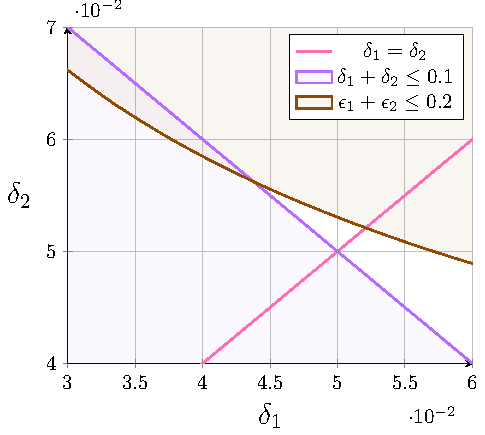
\includegraphics[width=0.75\linewidth]{avoir/images/concrete-example-tikz}
%    \resizebox{0.75\linewidth}{!}{
%                \input{images/concrete-example-tikz}
%    }
    \caption{\AVOIRmethodname{} finds a solution for a \textit{theoretical} scenario with $\delta_1 + \delta_2 \leq \Delta$ under constraint $\epsilon_1 + \epsilon_2 \leq \epsilon_T$. No solution exists with additional constraint $A_\delta: \delta_X = \delta_Y = \Delta/2$ - common assumption in prior work.}
    \label{fig:theoretical-example}
\end{figure}


